\documentclass[12pt]{article}

\usepackage{sbc-template}

\usepackage{graphicx,url}

\usepackage[brazil]{babel}   
%\usepackage[latin1]{inputenc}  
\usepackage[utf8]{inputenc}  
% UTF-8 encoding is recommended by ShareLaTex

\usepackage{mdframed}
\usepackage{minted}
\usepackage{hyperref}
\usepackage{amssymb}
\usepackage{amsmath}
     
\sloppy

\title{Trabalho Prático 3 - Redes Neurais Artificiais}

\author{Hugo Araujo de Sousa}

\address{
  Computação Natural (2017/2) \\
  Departamento de Ciência da Computação \\
  Universidade Federal de Minas Gerais (UFMG)
  \email{hugosousa@dcc.ufmg.br}
}

\begin{document} 

\maketitle
     
\begin{resumo}
  Nesse trabalho são explorados conceitos relacionados a redes neurais,
  colocando-os em prática através da utilização da biblioteca Keras com Tensorflow, 
  que nos permite abordar um problema de classificação.
\end{resumo}

\section{INTRODUÇÃO}

Dentro da área de Computação Natural, o campo de Redes Neurais Artificiais
tem como objetivo a criação de modelos computacionais inspirados pelo
conhecimento que temos sobre como funciona o sistema nervoso, mais
especificamente, na estrutura e função dos neurônios no cérebro
\cite{clevalg}.

Dessa forma, uma Rede Neural Artificial é uma coleção de neurônios
artificiais que são conectados a fim de se realizar alguma computação
em padrões de entrada para gerar padrões de saída. Esses neurônios,
então, se adaptam, modificando sua estrutura interna ao longo do tempo.
Geralmente, essa modificação se dá através da atualização dos pesos
das conexões entre os neurônios da rede. Esse processo define o
aprendizado da rede neural, que então se torna, com o tempo, cada
vez mais adaptada na tarefa de gerar o padrão de saída correto de 
acordo com a entrada.

No trabalho em questão, usaremos a biblioteca Keras 
\footnote{\url{https://keras.io/}} com Tensorflow
\footnote{\url{https://www.tensorflow.org/}}, que juntas fornecem
implementações de redes neurais já prontas para uso. A partir dessas 
duas bibliotecas, o problema a ser resolvido será o de classificação
de um conjunto de dados específico.

Esse conjunto de dados reúne informações de 1429 proteínas, descritas
por 8 atributos (números reais). Para cada uma dessas proteínas, a sua
classe se refere à parte da célula em que a proteína se encontra.
Ao todo, existem 7 classes possíveis, descritas na Tabela
\ref{tab:classes}.

\begin{table}[h]
	\centering
	\begin{tabular}{|c|c|}
		\hline
		\textbf{Classe} & \textbf{Descrição} \\ \hline
		\textbf{CYT} & Citoplasma \\ \hline
		\textbf{MIT} & Mitocôndria \\ \hline
		\textbf{ME1} & Uma membrana específica da célula \\ \hline
		\textbf{ME2} & Uma membrana específica da célula \\ \hline
		\textbf{ME3} & Uma membrana específica da célula \\ \hline
		\textbf{EXC} & Exterior da célula \\ \hline
		\textbf{NUC} & Núcleo da célula \\ \hline
	\end{tabular}
	\caption{\label{tab:classes} Classes que descrevem a posição
	das proteínas em uma célula.}
\end{table}

Portanto, a rede neural criada será alimentada com os dados dessa base e,
ao longo do tempo, tentará aprender os padrões que determinam a saída
da mesma, isto é, dado um conjunto de 8 atributos de uma proteína, a
rede deve dizer qual é a posição que essa proteína ocupa na célula (
representada pela classe, dentre as 7 descritas acima).

\section{MODELAGEM}

A modelagem do problema de classificação em questão, utilizando redes
neurais implementadas através da biblioteca Keras com Tensorflow é 
mostrada nessa seção.

\subsection{Arquitetura}

Para modelar esse problema, o primeiro passo é determinar qual o tipo
da rede neural a ser construída - existem vários tipos de arquitetura
de redes neurais diferentes.

Para o trabalho em questão, optou-se por simplicidade em termos de
representação, o que, por sua vez, acarreta em maior controle sobre 
a estrutura da rede e de seu funcionamento. Dessa forma, a arquitetura
escolhida foi a \textit{Multilayer Perceptron - MLP} (Perceptron de
múltiplas camadas) -, que é uma versão da rede \textit{Perceptron} 
generalizada para conter múltiplas camadas escondidas de neurônios.
A Figura \ref{fig:mlp} mostra a estrutura da rede MLP.

\begin{figure}[h]
  \centering
  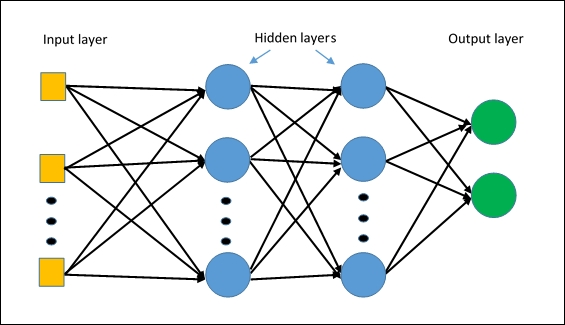
\includegraphics[width=1\textwidth]{mlp.jpg}
  \caption{Estrutura da rede \textit{Multilayer Perceptron}. Vemos
  que, além das camadas de entrada e saída, a rede também pode
  apresentar um número arbitrário de camadas escondidas de neurônios.
  O número de neurônios em cada camada também pode ser escolhido
  arbitrariamente.}
  \label{fig:mlp}
\end{figure}

O número de camadas escondidas e número de neurônios em cada camada
utilizados no trabalho foram definidos experimentalmente, como mostrado
na Seção \ref{sec:exp}.

De forma geral, temos que a saída que um neurônio produz consiste na
soma ponderada (pelos pesos) de suas entradas, além de um valor de
\textit{bias}.

\begin{displaymath}
	Saida = \sum_{} (Pesos * Entradas) + Bias
\end{displaymath}

Além disso, essa saída passa por uma função de ativação antes de 
servir como entrada para os neurônios da camada seguinte. Essa
função de ativação determina se e quanto um neurônio deve contribuir
na rede, de acordo com os valores que gera.

\subsection{Inicialização de Pesos}

Uma decisão importante é a de como inicializar os pesos na rede. Sabemos
que se uma camada escondida tem um grande número de entradas, pequenas
mudanças nos pesos podem causar grandes alterações nas saídas dessa
camada. Uma forma de contornar isso é tornar os pesos iniciais da rede
proporcionais ao número de entradas. Para esse trabalho, optou-se por
inicializar os pesos proporcionalmente à raiz quadrada do número de
entradas nas camadas. Na biblioteca Keras, pode-se fazer isso adicionando
o argumento \textit{kernel\_initializer='lecun\_uniform'} ao construtor
de uma nova camada.

\subsection{Funções de Ativação}

Como mencionado, o processo de ativar um neurônio é fundamental para o
funcionamento correto da rede neural artificial. Dessa forma, é uma
decisão importante escolher qual função de ativação utilizar nas camadas
da rede. Existem muitas opções e a escolha deve levar em consideração
o tipo de problema a ser resolvido, além dos conhecimentos sobre os 
padrões de entrada\cite{principe2000neural}. Para o trabalho em questão, duas funções foram escolhidas, uma para as camadas escondidas e uma
para a camada de saída.

Para camadas escondidas, a função ReLU foi escolhida, uma vez que
preserva algumas propriedades interessantes de funções lineares e
faz com que a otimização com descida do gradiente seja fácil
\cite{Goodfellow-et-al-2016}.

\begin{equation}
	RELU(x) = 
	\begin{cases}
		0, & \text{if} ~ x < 0 \\
		1, & \text{if} ~ x \geq 0
	\end{cases}
\end{equation}

Já para a camada de saída, a função escolhida foi a Sotfmax, que 
apresenta resultados geralmente bons para problemas de classificação
multi classe. Essa função transforma as saídas de cada neurônio
para um valor entre $ 0 $ e $ 1 $, como uma função sigmoide. Além
disso, ela também faz com que a soma total das saídas seja igual a 
$ 1 $.

\subsection{Função de Custo}

A rede implementada no trabalho utiliza o conceito de
\textit{back-propagation}, com o qual os erros da saída da camada
de saída são passados de volta para os neurônios internos, que usam
esses erros para calcular seus próprios erros e atualizar seus pesos.
Esse algoritmo é baseado na otimização de uma função de custo através
do método de descida do gradiente. Dessa forma, é também uma decisão
de implementação escolher a função de custo do algoritmo. Para esse
trabalho, a função escolhida foi a \textit{cross-entropy}

\subsection{Validação Cruzada}

A fim de garantir que os resultados de generalização da rede não estejam
sendo obtidos ao acaso, foi implementado um sistema de validação cruzada
de 3 partições. Nesse sistema, o conjunto de dados de entrada é separado
em 3 partes, sendo que, a cada momento, duas delas são usadas para
treino e a parte restante para teste.

\subsection{Codificação da Saída}

Tendo em vista que os dados de entrada apresentam as classes de saída
como strings, foi necessário transformá-las para alimentar a rede neural.
Essas strings que representam as classes foram codificadas utilizando
o sistema de variáveis categóricas distribuídas. Dessa forma, cada uma
delas foi transformada em um vetor de zeros e uns.

\section{ESTRUTURA DO PROJETO E EXECUÇÃO}

O trabalho foi implementado utilizando-se a linguagem Python 3. Como já
mencionado, as redes neurais artificiais foram criadas através da
biblioteca Keras com Tensorflow.

O projeto está estruturado em $ 4 $ diretórios, como definidos abaixo:

\begin{itemize}
	\item \textbf{doc:} Contém a documentação do trabalho.
	\item \textbf{src:} Arquivo executável que lê os dados de entrada
	e cria a rede neural artificial com base nos argumentos passados
	na linha de comando para resolver o problema de classificação.
	\item \textbf{input:} Base de dados de entrada.
	\item \textbf{tests:} Contém os resultados dos testes executados
	durante a fase de experimentação.
\end{itemize}

Para executar o programa, basta executar o seguinte comando no
diretório raiz do projeto:

\begin{center}
	tp3.py [-h] [-e EPOCHS] [-l HLAYERS] [-n NEURONS] [-b BATCHSIZE]
	              [-s RSEED] [-r LRATE] [-d LRDECAY]
	              arquivo\_entrada arquivo\_saida
\end{center}

\begin{itemize}
	\item \textbf{Argumentos posicionais:}

	\begin{itemize}
		\item input\_filename: Nome do arquivo de entrada.
	 	\item output\_filename: Nome do arquivo de saída.
	\end{itemize}

	\item \textbf{Argumentos opcionais:}

	\begin{itemize}
		\item -h, --help: Mostra uma mensagem de ajuda e termina
		execução.
		\item -e EPOCHS: Executa o aprendizado da rede neural artificial
		por um número EPOCHS de épocas.
		\item -l HLAYERS: Define o número de camadas escondidas como 
		HLAYERS.
		\item -n NEURONS: Faz com que cada camada escondida tenha
		um número NEURONS de neurônios.
		\item -b BATCHSIZE: Define BATCHSIZE como o tamanho dos
		batches usados no treinamento da rede.
		\item -r LRATE: Define a taxa de aprendizado da rede como LRATE.
		\item -d LRDECAY: Define a taxa de decaimento da taxa de
		aprendizado como LRDECAY.
		\item -s RSEED: Define RSEED como a semente para geração de 
		números aleatórios durante a execução do programa.
	\end{itemize}
\end{itemize}

\section{EXPERIMENTOS} \label{sec:exp}

A fim de verificar o comportamento da rede de acordo com os diversos
parâmetros do programa, uma série de experimentos foi realizada. Para
cada um deles, um parâmetro foi variável (aquele que buscava-se 
determinar), enquanto os outros foram mantidos fixos.
Além disso, para cada configuração de parâmetros, o programa foi
executado com $ 10 $ sementes diferentes, obtendo-se assim, ao final
de cada experimento, a média dos valores de cada execução.
Todos os testes foram executados em um computador i7-5500U CPU @ 
$ 2.40 $ GHz x 4, com Ubuntu 14.04 e $ 7.7 $ GB de memória RAM.

\subsection{Experimento 1 - Número de neurônios}

O primeiro experimento serviu para determinar o número de neurônios a ser
utilizado em cada camada escondida da rede. Para isso, os parâmetros
foram utilizados como descrito na Tabela \ref{tab:exp1} e o resultado
do experimento é mostrado na Figura \ref{fig:exp1}.

\begin{table}[h]
	\centering
	\begin{tabular}{|c|c|}
		\hline
		\textbf{Parâmetro} & \textbf{Valor(es)} \\ \hline
		e & 100 \\ \hline
		l & 1 \\ \hline
		n & 8, 16, 32, 64, 128 \\ \hline
		b & 10 \\ \hline
		r & 0.05 \\ \hline
		d & 0 \\ \hline
		s & 10 para cada n \\ \hline
	\end{tabular}
	\caption{\label{tab:exp1} Valores de parâmetros para o Experimento
	1.}
\end{table}

\begin{figure}[h]
  \centering
  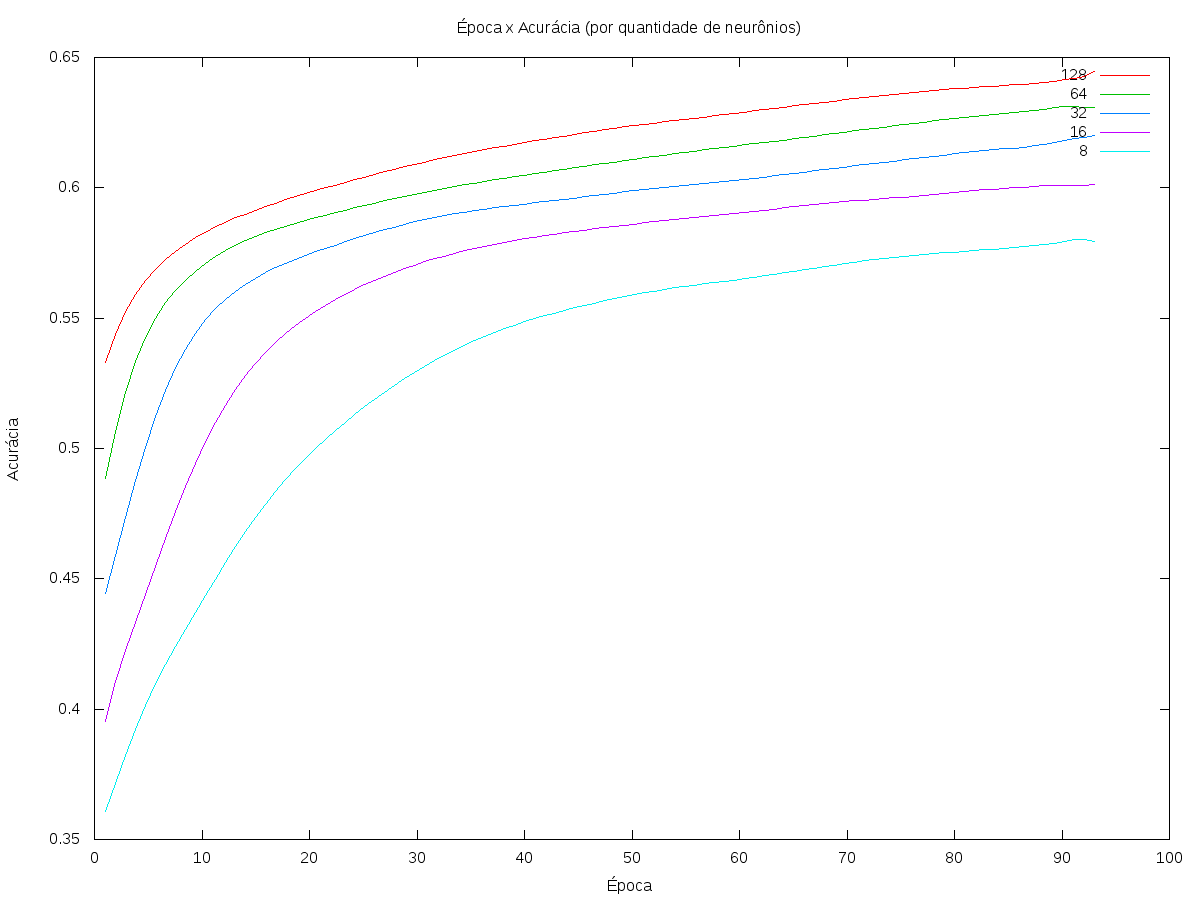
\includegraphics[width=1\textwidth]{../tests/1-neurons/graph.png}
  \caption{Experimento 1 - Época x Acurácia da rede para diferentes
  números de neurônios na camada escondida.}
  \label{fig:exp1}
\end{figure}

Vemos então que o aumento no número de neurônios sempre acarreta em uma
convergência mais rápida, além da rede conseguir alcançar valores mais
altos de acurácia para o mesmo número de épocas. Nessa configuração,
uma boa escolha para número de neurônios é então o valor $ 32 $ que,
quando comparado com os outros valores, possui uma velocidade de
convergência razoável, além de não perder muito em acurácia em relação
aos valores de $ 64 $ e $ 128 $ neurônios.

\subsection{Experimento 2 - Número de camadas escondidas}

Uma vez determinado o número de neurônios a utilizar, precisamos
determinar quantas camadas escondidas usar na rede. De forma análoga
ao Experimento 1, os parâmetros utilizados nesse teste são mostrados
na Tabela \ref{tab:exp2} e o resultado do experimento é apresentado
na Figura \ref{fig:exp2}.

\begin{table}[h]
	\centering
	\begin{tabular}{|c|c|}
		\hline
		\textbf{Parâmetro} & \textbf{Valor(es)} \\ \hline
		e & 200 \\ \hline
		l & 1, 2, 4, 6, 8 \\ \hline
		n & 32 \\ \hline
		b & 10 \\ \hline
		r & 0.05 \\ \hline
		d & 0 \\ \hline
		s & 10 para cada l \\ \hline
	\end{tabular}
	\caption{\label{tab:exp2} Valores de parâmetros para o Experimento
	2.}
\end{table}

\begin{figure}[h]
  \centering
  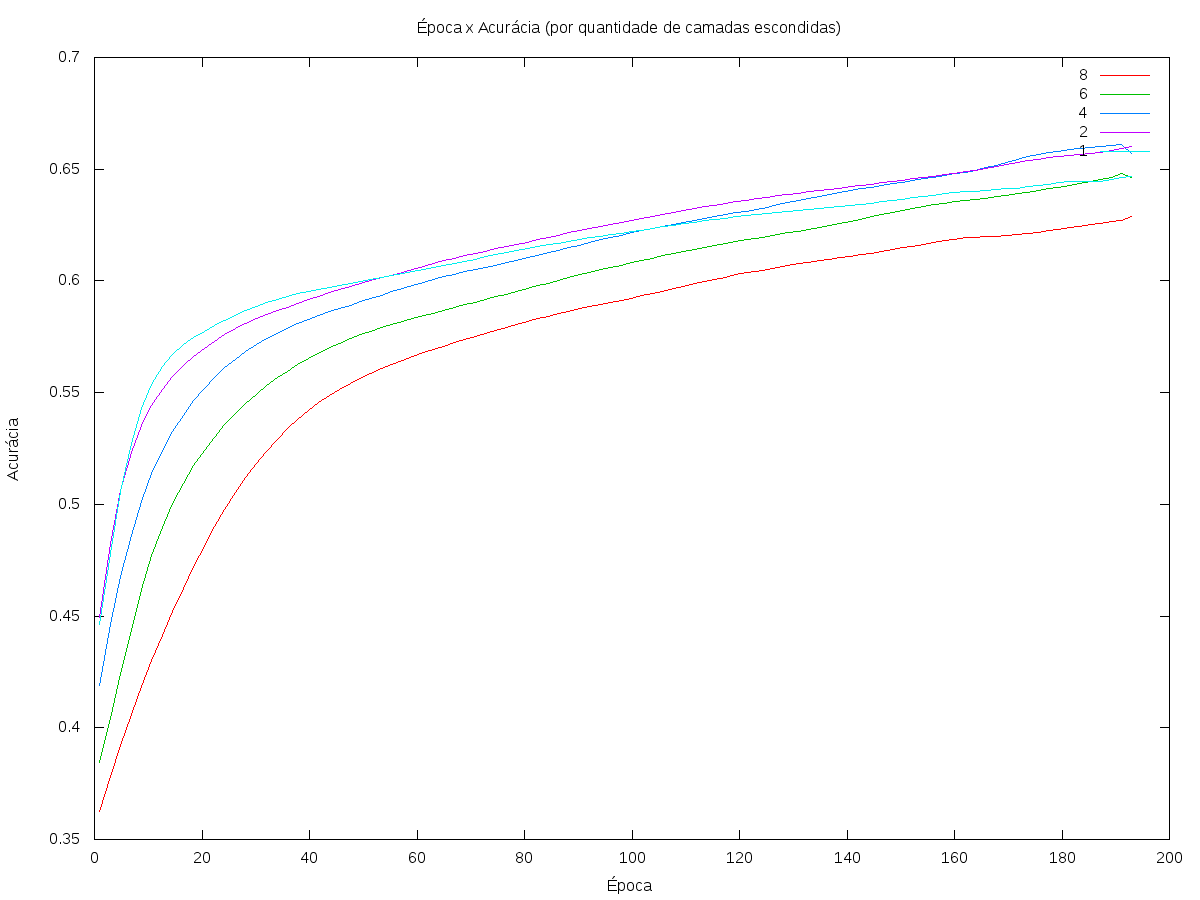
\includegraphics[width=1\textwidth]{../tests/2-layers/graph.png}
  \caption{Experimento 2 - Época x Acurácia da rede para diferentes
  números de camadas escondidas.}
  \label{fig:exp2}
\end{figure}

Para esse experimento podemos verificar que com $ 4 $ camadas escondidas,
a rede consegue o maior valor de acurácia ao final das épocas, além 
de não apresentar convergência imatura, quando comparada com os valores
de $ 1 $ e $ 2 $ camadas.

\subsection{Experimento 3 - Taxa de aprendizado}

Com o número de camadas escondidas e número de neurônios em cada camada
determinados, o próximo parâmetro a definir é a taxa de aprendizado
da rede. Os parâmetros do experimento são mostrados na Tabela
\ref{tab:exp3} e os resultados do mesmo são apresentados na Figura
\ref{fig:exp3}.

\begin{table}[h]
	\centering
	\begin{tabular}{|c|c|}
		\hline
		\textbf{Parâmetro} & \textbf{Valor(es)} \\ \hline
		e & 200 \\ \hline
		l & 4 \\ \hline
		n & 32 \\ \hline
		b & 10 \\ \hline
		r & 0.05, 0.1, 0.2, 0.4, 0.6, 0.9 \\ \hline
		d & 0 \\ \hline
		s & 10 para cada r \\ \hline
	\end{tabular}
	\caption{\label{tab:exp3} Valores de parâmetros para o Experimento
	3.}
\end{table}

\begin{figure}[h]
  \centering
  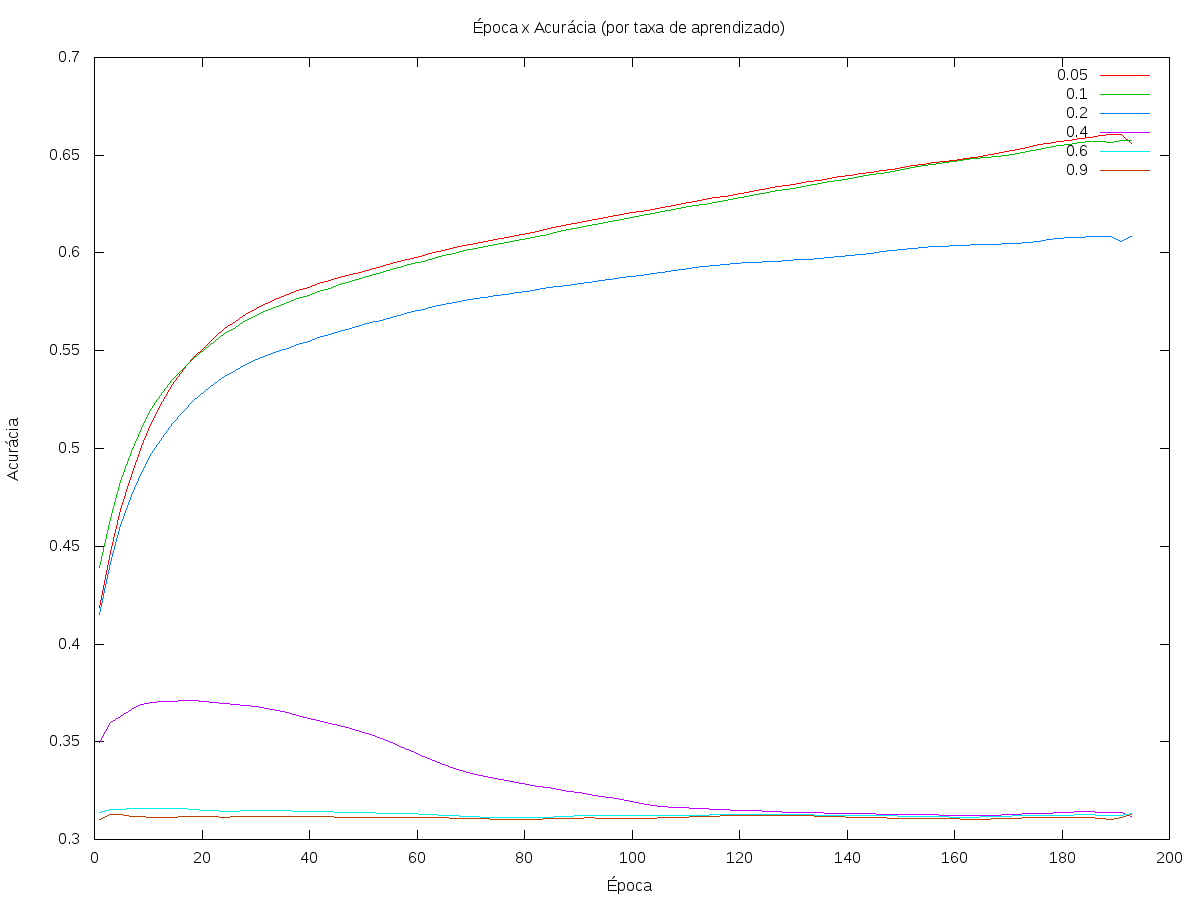
\includegraphics[width=1\textwidth]{../tests/3-lrate/graph.png}
  \caption{Experimento 3 - Época x Acurácia da rede para diferentes
  valores de taxa de aprendizado.}
  \label{fig:exp3}
\end{figure}

Com o resultado desse teste podemos verificar uma curiosa anomalia:
para valores a partir de $ 0.4 $ o desempenho da rede se torna 
extremamente ruim, sendo a mesma incapaz de aprender. A escolha fica
então entre os valores de $ 0.05 $ e $ 0.1 $, que atingem valores
muito próximos de acurácia. O desempate fica então pelo fator de
convergência, escolhendo-se assim o valor $ 0.05 $, para o qual a
convergência não ocorre tão rapidamente quanto com taxa de
aprendizado igual a $ 0.1 $.

\subsection{Experimento 4 - Taxa de decaimento da taxa de aprendizado}

Além de fixar a taxa de aprendizado, podemos verificar o que acontece
quando a fazemos variar com o tempo. Para isso, é possível
especificar uma taxa de decaimento para a taxa de aprendizado, que é
então reduzida automaticamente ao longo das épocas de treino.
No experimento 4 isso foi feito com os parâmetros mostrados na Tabela
\ref{tab:exp4}, obtendo os resultados mostrado na Figura 
\ref{fig:exp4}.

\begin{table}[h]
	\centering
	\begin{tabular}{|c|c|}
		\hline
		\textbf{Parâmetro} & \textbf{Valor(es)} \\ \hline
		e & 200 \\ \hline
		l & 4 \\ \hline
		n & 32 \\ \hline
		b & 10 \\ \hline
		r & 0.05 \\ \hline
		d & 0.01, 0.02, 0.04, 0.08, 0.1 \\ \hline
		s & 10 para cada d \\ \hline
	\end{tabular}
	\caption{\label{tab:exp4} Valores de parâmetros para o Experimento
	4.}
\end{table}

\begin{figure}[h]
  \centering
  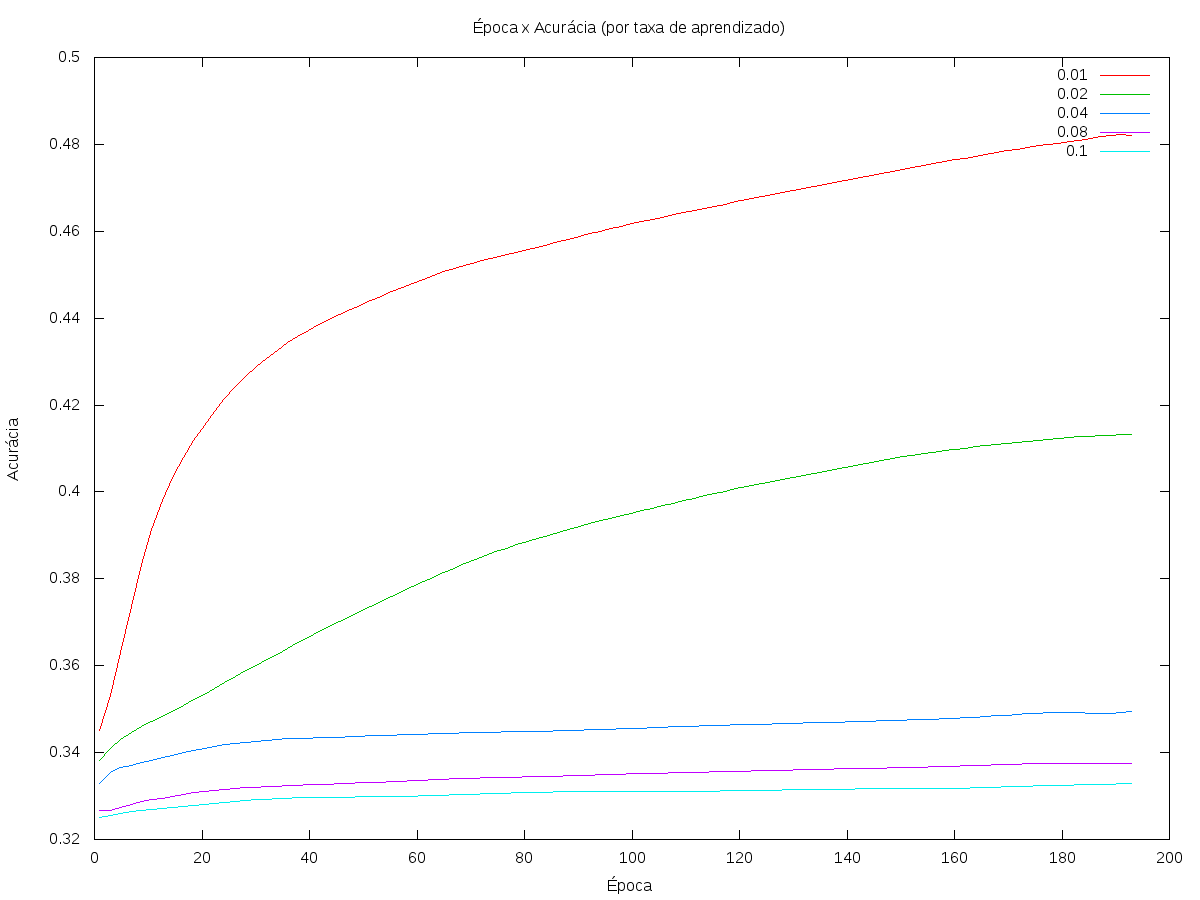
\includegraphics[width=1\textwidth]{../tests/4-lrdecay/graph.png}
  \caption{Experimento 4 - Época x Acurácia da rede para diferentes
  valores de decaimento taxa de aprendizado.}
  \label{fig:exp4}
\end{figure}

Aqui percebemos que, com uma taxa de decaimento para a taxa de
aprendizado, somente retardamos a convergência da rede. Nessa situação
optou-se por não utilizar uma taxa de decaimento, isto é, usar
$ d = 0 $.

\subsection{Experimento 5 - Tamanho de batch}

Em seguida, o objetivo foi comparar o treinamento da rede com o método
de descida de gradiente estocástico com o uso de mini-batches. Com
o uso de mini-batches de tamanho $ b $, os pesos da rede só são atualizados
após $ b $ exemplos serem alimentados à mesma, ao contrário da abordagem
tradicional onde cada exemplo atualiza os pesos ($ b = 1 $). Dessa forma,
o experimento procurou verificar o ganho a acurácia da rede para diferentes
valores de $ b $ e como o tempo computacional é afetado por esse parâmetro.
Os parâmetros do experimento são mostrados na Tabela \ref{tab:exp5} e os
resultados do mesmo são ilustrados nas Figuras \ref{fig:exp51} e
\ref{fig:exp52}.

\begin{table}[h]
	\centering
	\begin{tabular}{|c|c|}
		\hline
		\textbf{Parâmetro} & \textbf{Valor(es)} \\ \hline
		e & 200 \\ \hline
		l & 4 \\ \hline
		n & 32 \\ \hline
		b & {1, 1, 25, 50, 100} \\ \hline
		r & 0.05 \\ \hline
		d & 0 \\ \hline
		s & 10 para cada b \\ \hline
	\end{tabular}
	\caption{\label{tab:exp5} Valores de parâmetros para o Experimento
	5.}
\end{table}

\begin{figure}[h]
  \centering
  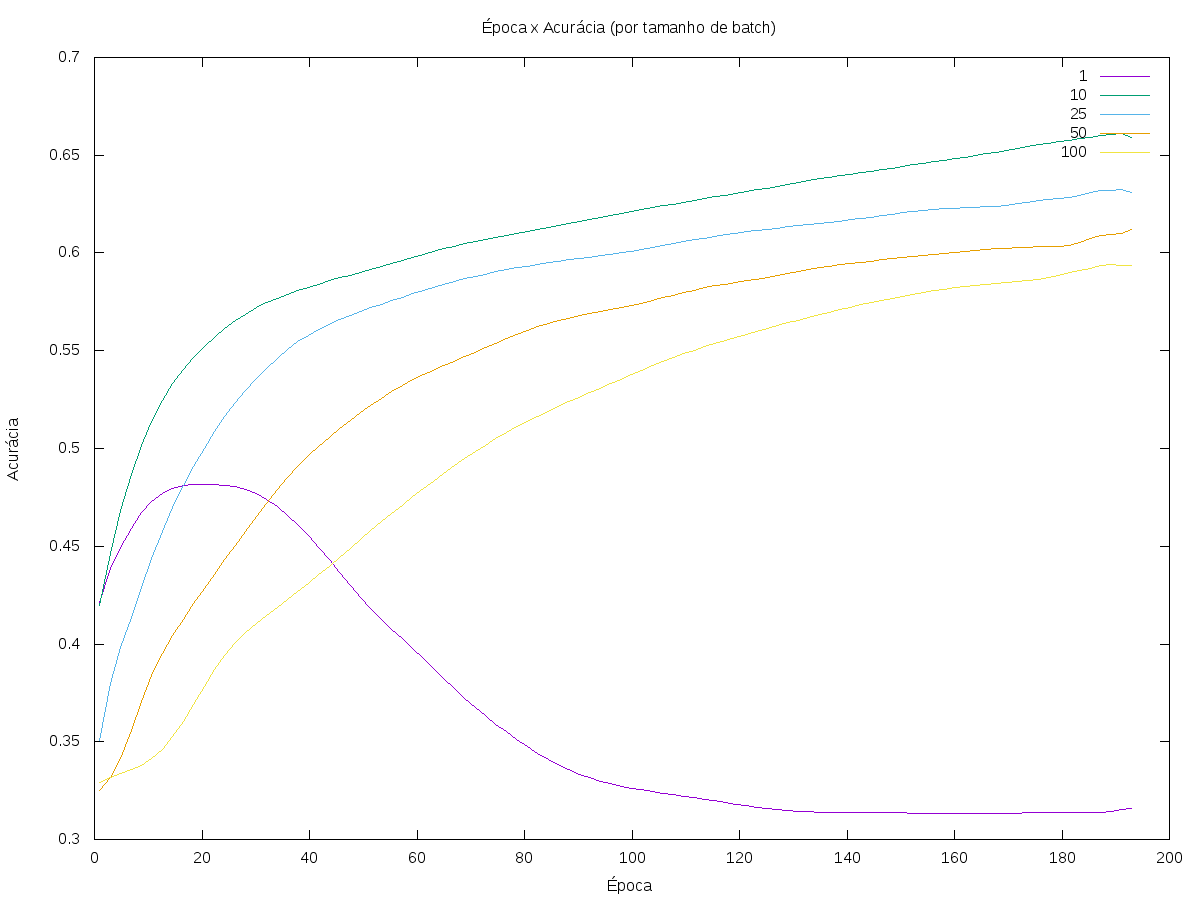
\includegraphics[width=1\textwidth]{../tests/5-batch/graph1.png}
  \caption{Experimento 5 - Época x Acurácia da rede para diferentes
  valores de tamanho de mini-batch.}
  \label{fig:exp51}
\end{figure}

\begin{figure}[h]
  \centering
  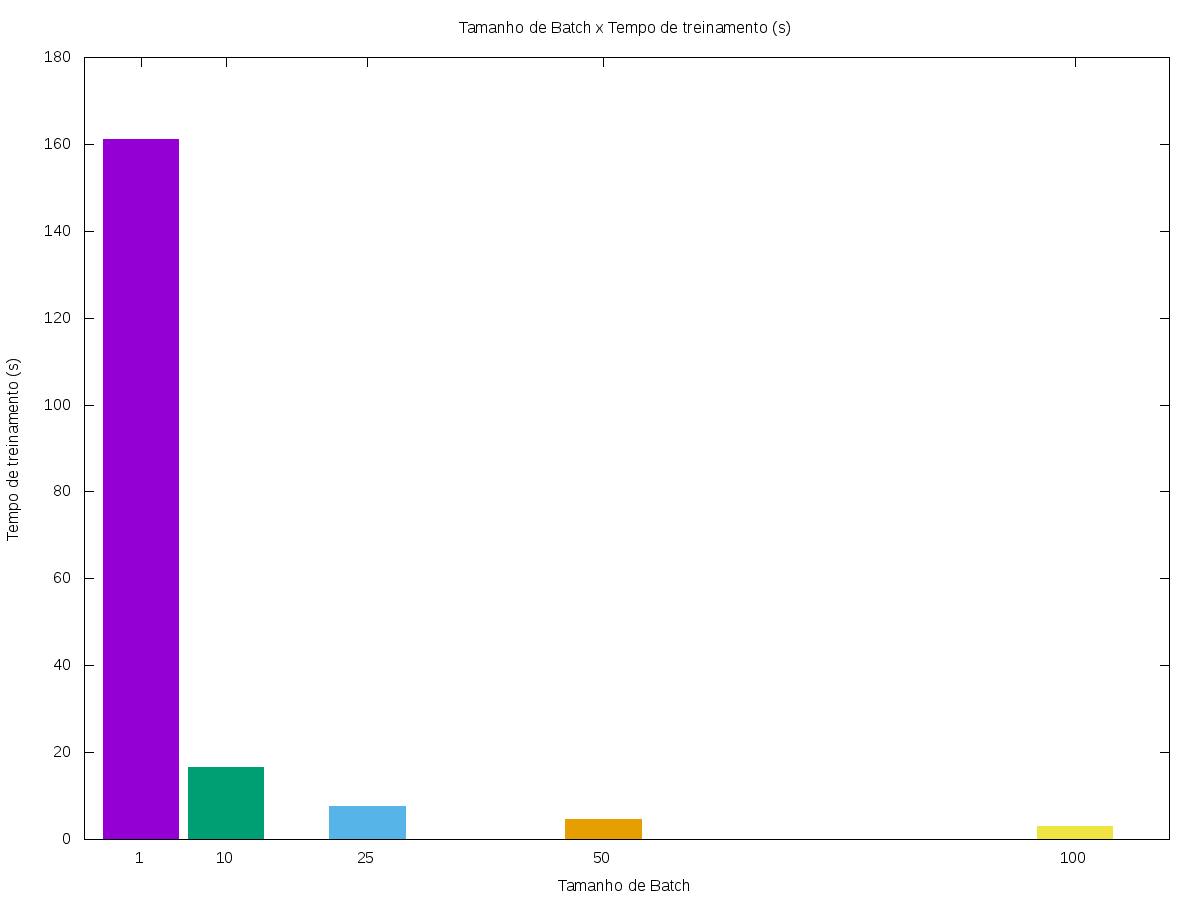
\includegraphics[width=1\textwidth]{../tests/5-batch/graph2.png}
  \caption{Experimento 5 - Tempo de treinamento x tamanho de mini-batch
  utilizado.}
  \label{fig:exp52}
\end{figure}

Na Figura \ref{fig:exp51} vemos que a convergência da acurácia da rede
se torna gradativamente mais lenta, quando variamos o tamanho do mini-batch
de $ 10 $ até $ 100 $. Além disso, vemos que com tamanho igual a $ 1 $
para mini-batch, a rede sofre uma anomalia que a impede de aprender ao longo
do tempo.

Em relação ao tempo de treinamento, vemos que esse decai de forma exponencial
com o aumento do tamanho do mini-batch. Sendo assim, o tamanho de mini-batch
escolhido é $ 10 $, uma vez que apresenta melhor custo benefício quando
comparamos acurácia obtida e tempo de treinamento.

\subsection{Experimento 6 - Overfitting}



\section{CONCLUSÃO}



\section{REFERÊNCIAS}

\bibliographystyle{sbc}
\bibliography{sbc-template}

\end{document}
